\documentclass[11pt]{article}
\usepackage[top=1in, bottom=1in, left=1in, right=1in]{geometry}

\usepackage{amsmath}
\usepackage{amssymb}
\usepackage{graphicx}

\usepackage{multicol}

\usepackage{enumerate}

\title{Quiz \#3, 9/10 \\ Math 156 (Calculus I), Fall 2024}
\date{}

\begin{document}

\maketitle

\thispagestyle{empty}

\vspace{-2cm}

Problem 1 is worth 8 points and Problem 2 is worth 2 points, for a total of 10 points. Remember to \emph{show your work} on all problems!

\begin{enumerate}
\item Consider the function $f(x)$ graphed below:
\[ 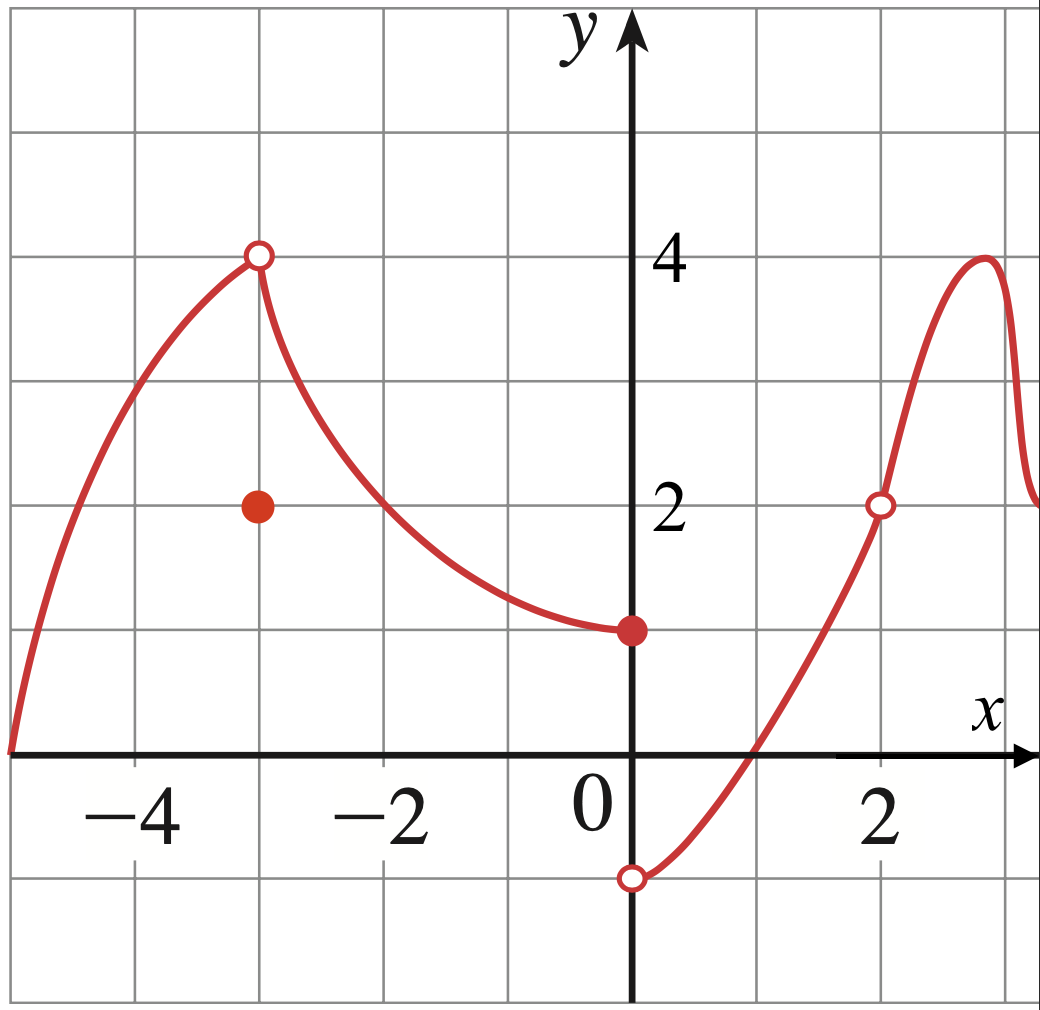
\includegraphics[width=2in]{quiz3.png}\]
For each of the following values of $a$: i) say what $\displaystyle \lim_{x \to a} f(x)$ is or state that it does not exist; ii) say what $f(a)$ is or state that it does not exist; iii) state whether $f(x)$ is continuous at $a$.
\begin{multicols}{2}
\begin{enumerate}
\item $a=-3$
\item $a=0$
\item $a=1$
\item $a=2$
\end{enumerate}
\end{multicols}

\vspace{5cm}

\item The position (in meters) at time $t$ (in seconds) of a car driving down a straight road is given by the function $f(t)$. What does the quantity $\displaystyle \lim_{t \to 7} \frac{f(t) - f(7)}{t-7}$ represent?

\end{enumerate}

\end{document}
